\section{Erfolgsbedingung und finale Auswertung}
\begin{wrapfigure}{l}{0.6\textwidth} 
	\centering
	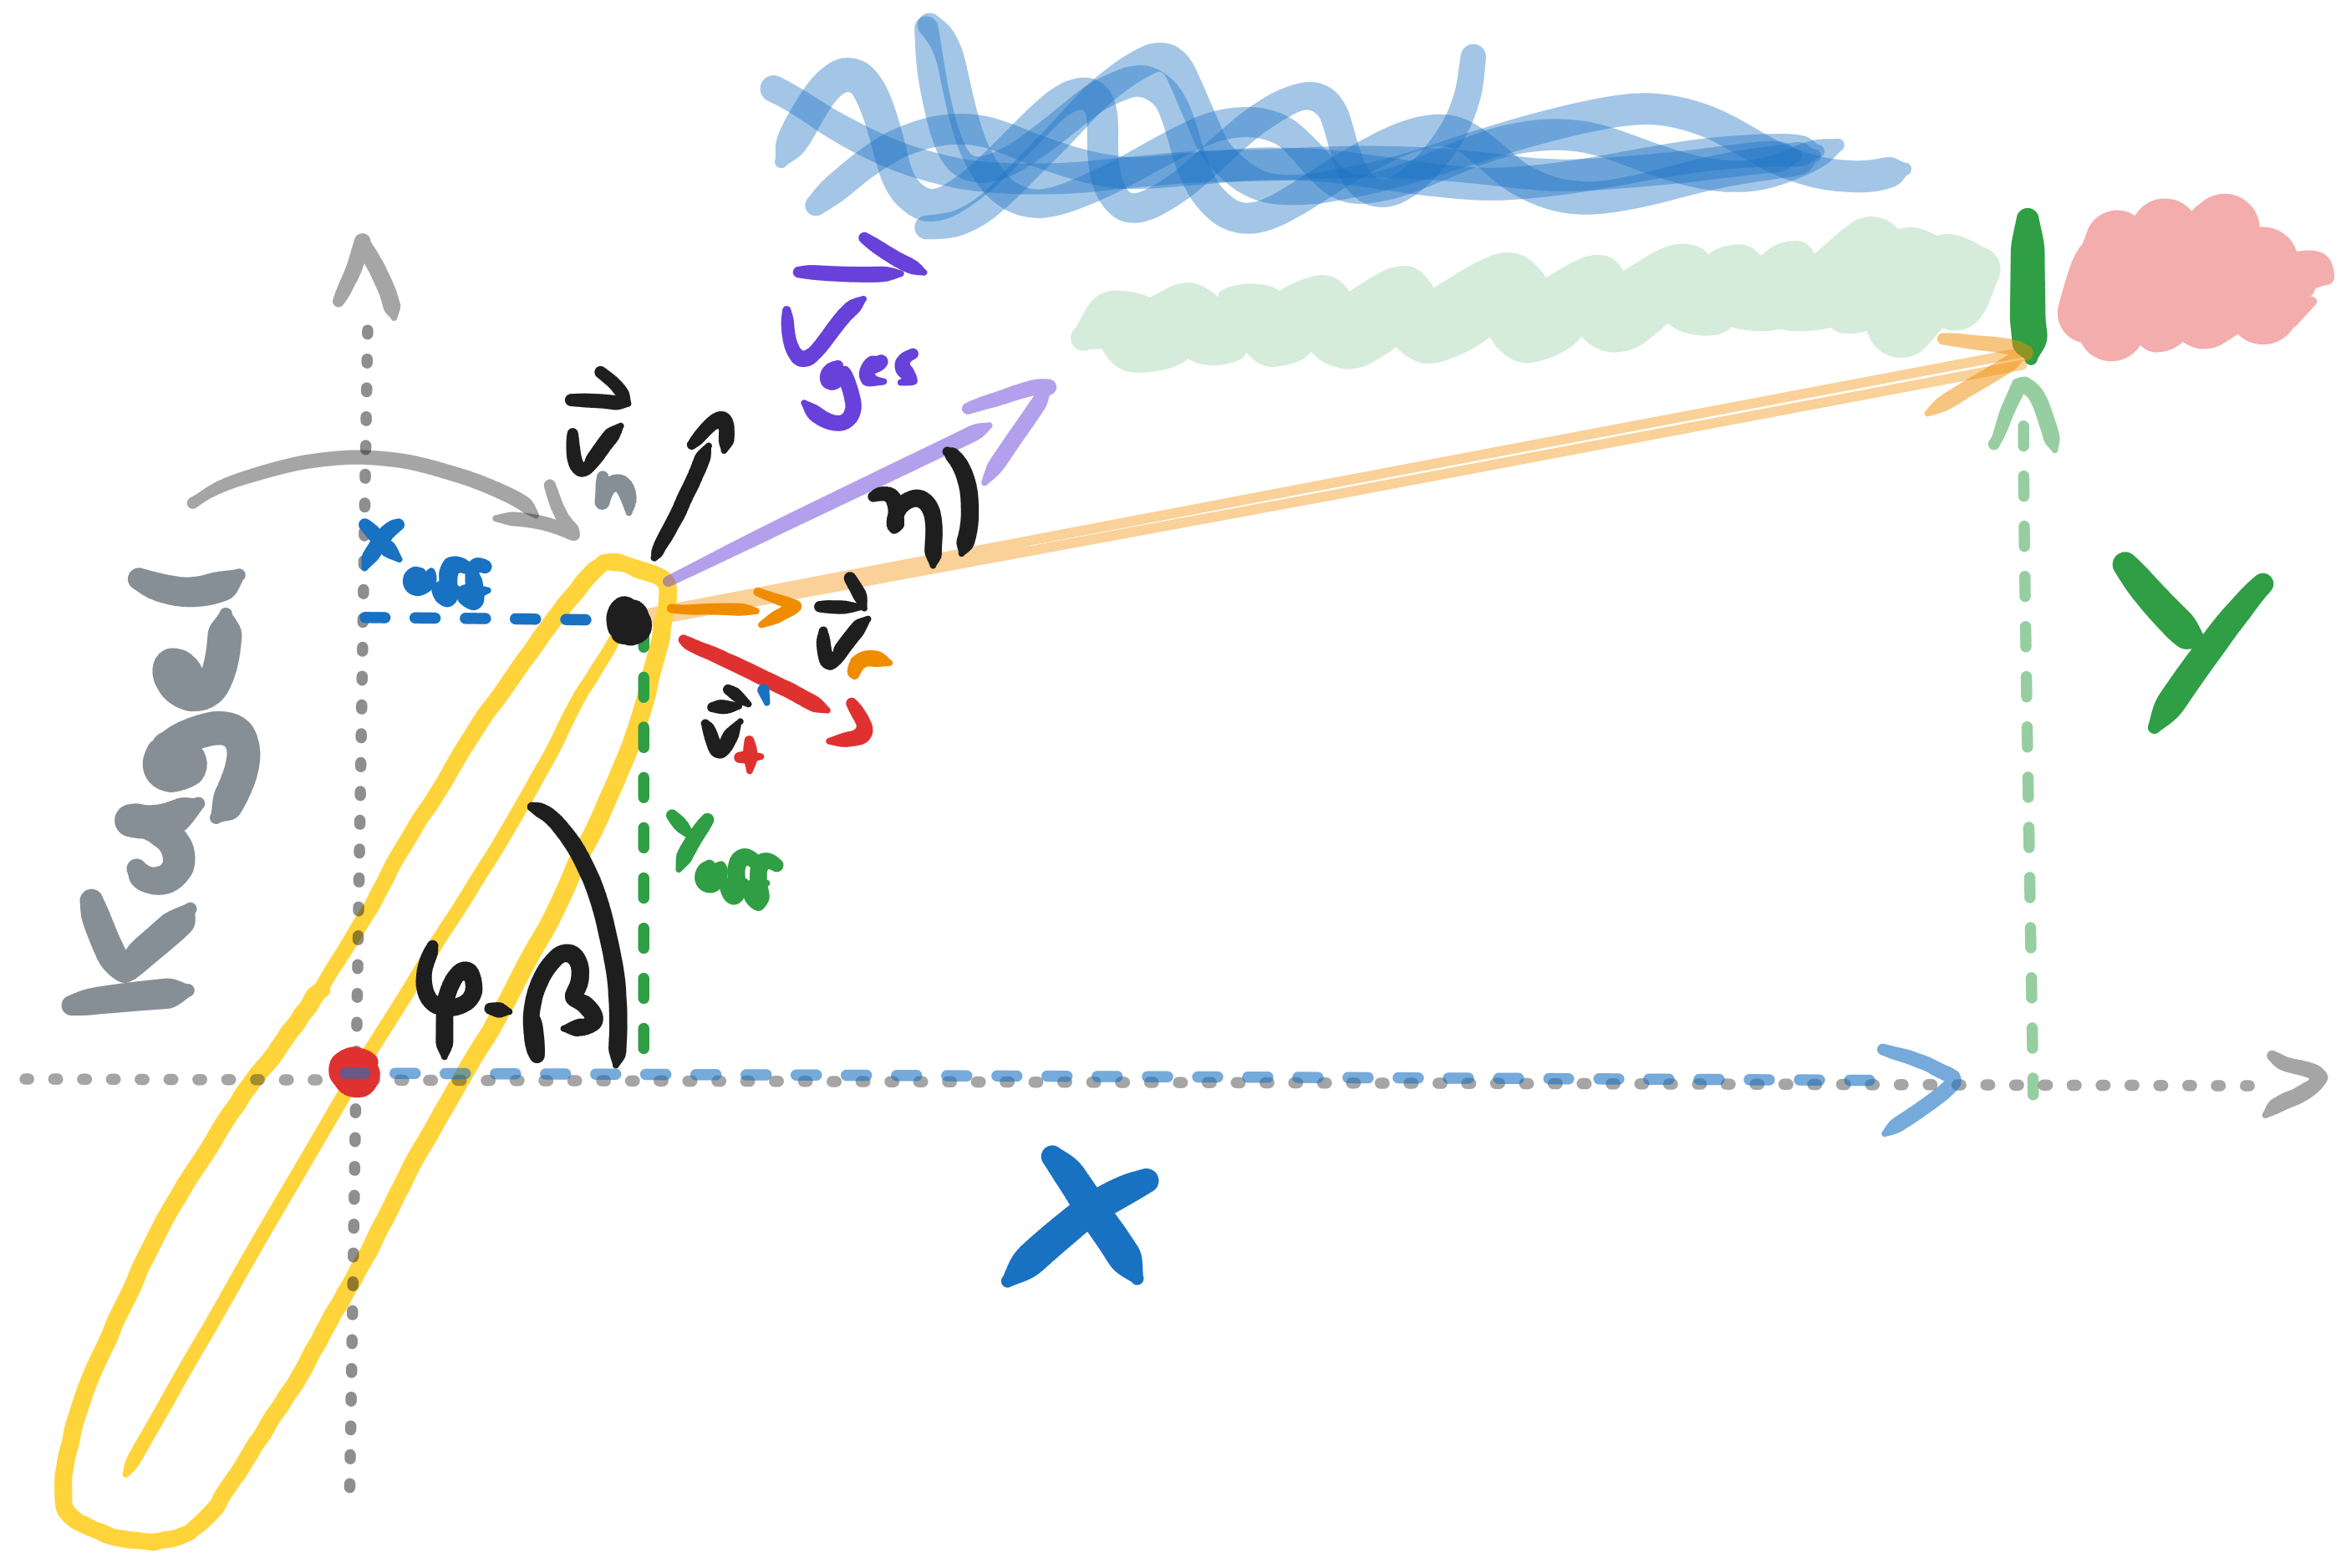
\includegraphics[width=0.58\textwidth]{resources/seq6/00-sketch-result.png}
	\vspace*{-5mm}
	\begin{flushright}
		{\scriptsize Eigenkreation; Gezeichnet in Excalidraw}
	\end{flushright}
	
	\captionsetup{
		labelfont=bf,
		textfont=footnotesize,
		skip=0pt
	}
	\caption{Skizze der Erfolgsbedingung aus Sequenz 5 in Draufsicht}
	\label{fig:06_sketch_result}
	%\vspace{-10pt}
\end{wrapfigure}
Die fünfte Sequenz markiert mit dem Eintauchen der Kugel den Abschluss unserer Untersuchungen. An dieser Stelle werden die Ergebnisse des vorherigen Abschnitts zusammengeführt und in Bezug zu den räumlichen Gegebenheiten gesetzt, um anschließend für den gegebenen Parametersatz eine finale Erfolgsprognose zu erstellen. 
\\
Es wird wieder der ursprüngliche und nicht rotierte metrische Raum betrachtet. 
\\
Unmittelbar nach der Kollision befindet sich die Kugel am selben Punkt wie das Gegengewicht des Krans: $P\!\left(\begin{smallmatrix} x_{\text{off}} \;= r \cdot \cos(\varphi-\beta) \\[2pt] y_{\text{off}} \;= r \cdot \sin(\varphi-\beta) \end{smallmatrix}\right)$
Anschließend können die drei unterschiedlichen Geschwindigkeitsvektoren, der unveränderte orthogonale, der reduzierte tangentiale sowie der neue, ursprünglich rotatorische, zum Gesamtvektor $\vec{v}_{\text{ges}} = \vec{v}_n + \vec{v}'_t + \vec{v}_r$ aufaddiert werden.
\\
Damit die Kugel vor dem Brückenende ins Wasser stürzt und nicht von der Brücke auf die Straße im Vatikan rollt, muss sie vor dem maximalen $x$-Wert, der für die Brückenlänge steht, einen $y$-Wert, stellvertretend für den Abstand zwischen Kugel und der zu durchbrechenden Brückenbrüstung, überschreiten. Dieser ist in \hyperref[fig:04_sketch-whole]{Abbildung~\ref*{fig:04_sketch-whole}} als grüner Schwellwert markiert.
\\
Die letztmögliche Bahn, die sie einschlagen kann, um gerade noch den grünen Bereich zu erreichen und ins Wasser zu fallen, ist durch die orangefarbene Linie vom Kollisionspunkt bis zur grünen Barriere zwischen dem grünen und roten Bereich dargestellt. Dieser Grenzwinkel $\eta$ lässt sich über die Komponenten der Strecke bestimmen: $\eta = \arctan\left(\tfrac{y-y_{\text{off}}}{x-x_{\text{off}}}\right)$
\\
Analog dazu ergibt sich der Winkel $\alpha$ des Gesamtgeschwindigkeitsvektors $\vec{v}_{\text{ges}}$ zur $x$-Achse aus dessen Komponenten: $\alpha = \arctan\left(\tfrac{v_{y,\text{ges}}}{v_{x,\text{ges}}}\right)$
\\
Die Erfolgsbedingung lautet somit $\alpha \geq \eta$, was bedeutet, dass der Geschwindigkeitsvektor oberhalb der orangefarbenen Grenzlinie liegen muss.
\\
Theoretisch existiert für die Orientierung auch eine obere Grenze, praktisch ist diese jedoch irrelevant, da derartige Werte unter realistischen Bedingungen nicht erreicht werden können.

\iffalse
Es ist zu beachten, dass die $\arctan$-Funktion nur Werte im Bereich $(-\frac{\pi}{2}, \frac{\pi}{2})$ liefert und somit nicht zwischen allen vier Quadranten unterscheiden kann. Für eine eindeutige Winkelbestimmung über den vollen Bereich $(-\pi, \pi]$ sollte die $\operatorname{atan2}$-Funktion verwendet werden:
\[\eta = \operatorname{atan2}(y-y_{\text{off}}, x-x_{\text{off}})\]
\[\alpha = \operatorname{atan2}(v_{y,\text{ges}}, v_{x,\text{ges}})\]



Diese Linie lässt sich ebenfalls als Vektor ausdrücken:
$\vec{s} = \left(\begin{smallmatrix} x-x_{\text{off}} \\[2pt] y-y_{\text{off}} \end{smallmatrix}\right)$
Anschließend kann der Vektor $\vec{s}$ mit dem Gesamtgeschwindigkeitsvektor $\vec{v}_{\text{ges}}$ verglichen werden. Dabei dient $\vec{s}$ als Referenzvektor, relativ zu welchem die Orientierung von $\vec{v}_{\text{ges}}$ bestimmt wird. Die Erfolgsbedingung ergibt sich aus dem orientierten Kreuzprodukt der beiden Vektoren:
\[\vec{s} \times \vec{v}_{\text{ges}} = (x-x_{\text{off}}) \cdot v_{y,\text{ges}} - (y-y_{\text{off}}) \cdot v_{x,\text{ges}} \geq 0\]
Ist diese Bedingung erfüllt, so verläuft der Winkel von $\vec{s}$ nach $\vec{v}_{\text{ges}}$ gegen den Uhrzeigersinn, was bedeutet, dass $\vec{v}_{\text{ges}}$ oberhalb von $\vec{s}$ liegt und die Kugel den grünen Bereich erreicht. 
\\
Der Betrag des Winkels $\eta$ zwischen den beiden Vektoren lässt sich mittels Skalarprodukt bestimmen:
\[\cos(\eta) = \frac{\vec{s} \cdot \vec{v}_{\text{ges}}}{|\vec{s}| \cdot |\vec{v}_{\text{ges}}|} = \frac{(x-x_{\text{off}}) \cdot v_{x,\text{ges}} + (y-y_{\text{off}}) \cdot v_{y,\text{ges}}}{|\vec{s}| \cdot |\vec{v}_{\text{ges}}|}\]
Das Skalarprodukt allein liefert jedoch keine Information über die Orientierung des Winkels. Durch Kombination beider Ausdrücke ergibt sich der orientierte Winkel:
\[\eta = \operatorname{sgn}\left(\vec{s} \times \vec{v}_{\text{ges}}\right) \cdot \arccos\left(\frac{\vec{s} \cdot \vec{v}_{\text{ges}}}{|\vec{s}| \cdot |\vec{v}_{\text{ges}}|}\right)\]
wobei die Signum-Funktion das Vorzeichen des Kreuzprodukts liefert und somit die Drehrichtung kodiert. Für ein erfolgreiches Eintauchen muss $\eta \geq 0$ gelten. Theoretisch existiert für die Orientierung auch eine obere Grenze, praktisch ist diese jedoch irrelevant, da derartige Werte unter realistischen Bedingungen nicht erreicht werden können.

\fi